\subsection{Simulated data}

The results presented in this section will be based on simulated data.
The main advantage to work with simulated data in our situation, is the possibility to have a ground truth to compare our results to.
However, we do not have a baseline method to compare the performances of our algorithm with.
For this reason, the results presented will focus on the capacity of our algorithm to converge toward a solution.

To simulate the data, two steps are necessary: first, the simulation of the task timestamps $t^{(p)} = \braces{t^{(p)}_1, \dots, t^{(p)}_{n_p}}$, that allows to determine an intensity function $\lambda_{k,p}$, and second, thanks to this function, the simulation of the atom's activation's timestamps $\mathcal{A}_k$ using the simulation algorithm of one-dimensional nonhomogeneous Poisson process previously introduced (Algo.~\ref{algo:1d_inhomogenous_pp}).
To simulate the task timestamps, we simply generate regular timestamps during the entire duration of the experimentation $T$ with a given interval (inter stimulus interval), \SI{1.2}{\second}, that will be denoted by the variable \texttt{isi}.
Then, we randomly select a percentage of those timestamps to keep, e.g., \SI{80}{\percent}.
This percentage is denoted in the following by the variable \texttt{n\_tasks}\footnote{This variable is denoted \texttt{n\_tasks} and not \texttt{percent\_tasks} as in the implementation, one can specify directly the exact number of tasks to keep. A percentage is only taken into account if the variable is set to a number less than 1.}.

In the following, we call hyper-parameters the variables $T$, \texttt{isi}, \texttt{n\_tasks} and the truncation values $a$ and $b$ of the kernel, as they are not parameters that are learnt by the model.
The parameters $\mu$, $\alpha$, $m$ and $\sigma$, that are learnt by the model, will simply be called parameters or variables, interchangeably.

For the first experimentation, we are interested in determining to what extent the EM algorithm makes it possible to retrieve the true values of the parameters, and at what speed.
In other words, we are looking to find out whether or not the algorithms converges, both in the loss function and parameter values.
We fix the hyper-parameters at the following values, in order to generate data similar to an M/EEG recording: $T = \SI{4}{\minute}$, $\texttt{isi}=\SI{1.2}{\second}$, $\texttt{n\_tasks} = \SI{80}{\percent}$, $\intervalleFF{a}{b} = \intervalleFF{30}{800}\times \SI{e-3}{\second}$.
The loss history and the parameters recovery are respectively presented in Figures~\ref{fig:history_loss_1} and \ref{fig:history_params_1}.
Other results of similar experiences are presented in Appendix~\ref{annexe:extra_results_simulated}.

\begin{figure}[h!]
    \centering
    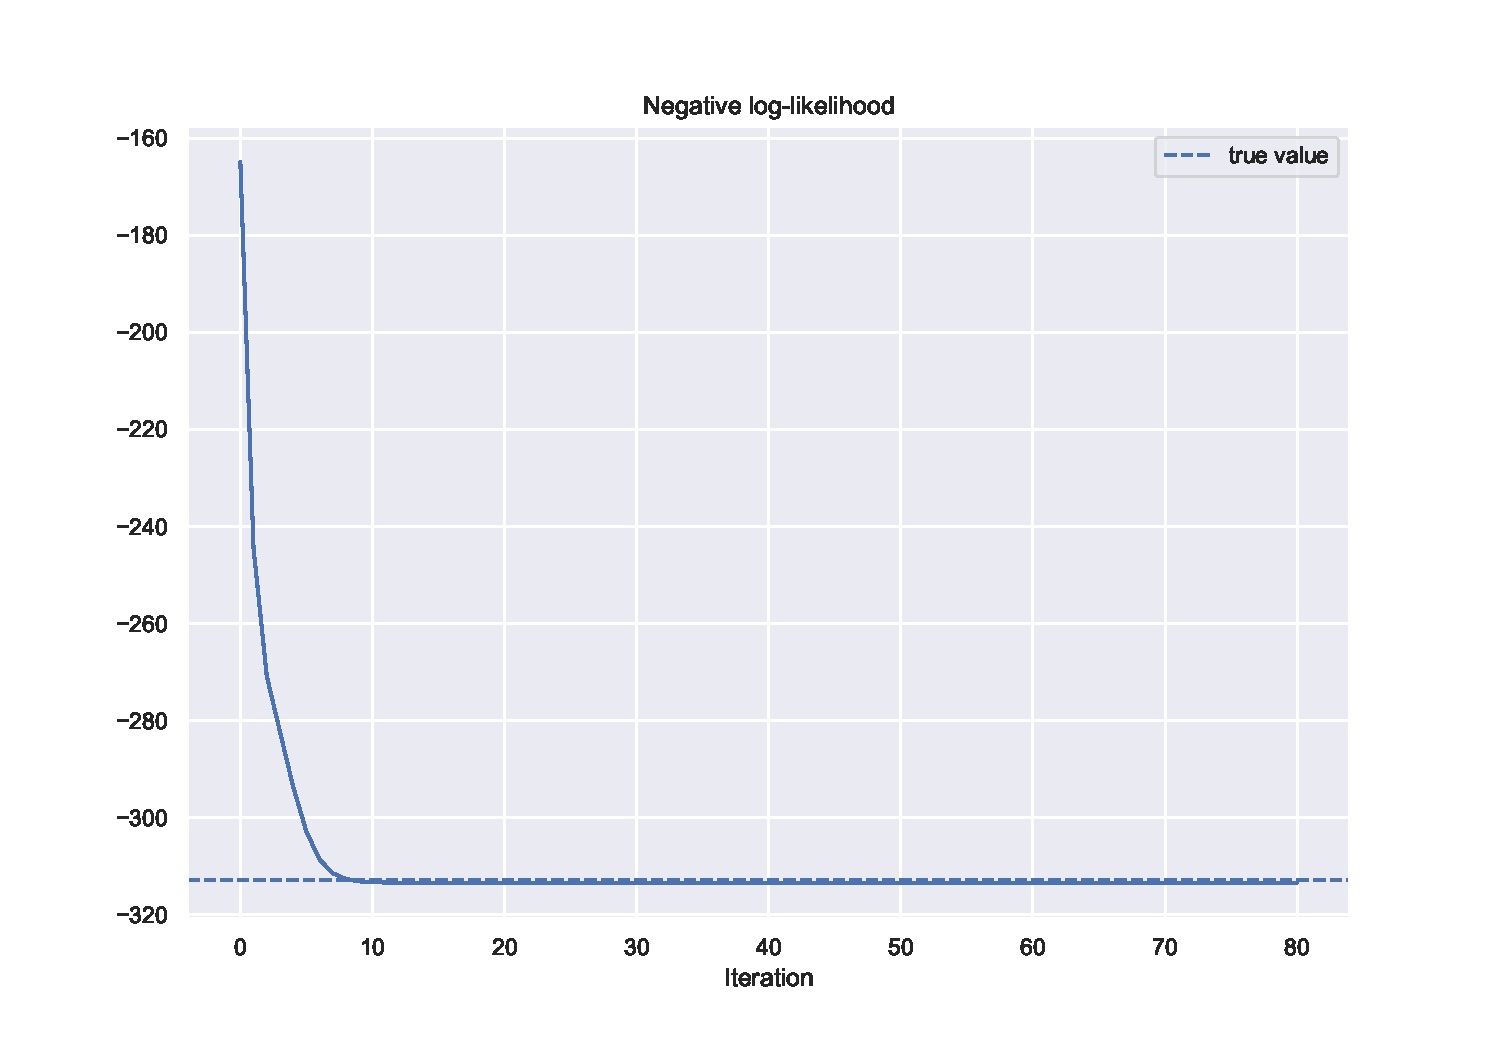
\includegraphics[width=0.9\textwidth]{pics/results/history_loss.pdf}
    \caption{Loss history over 80 iterations with a \textit{smart} initialisation, on simulated data with $T = \SI{4}{\minute}$, ${\texttt{isi}=\SI{1.2}{\second}}$, $\texttt{n\_tasks} = \SI{80}{\percent}$, $\intervalleFF{a}{b} = \intervalleFF{30}{800}\times \SI{e-3}{\second}$.}
    \label{fig:history_loss_1}
\end{figure}

\begin{figure}[h!]
    \centering
    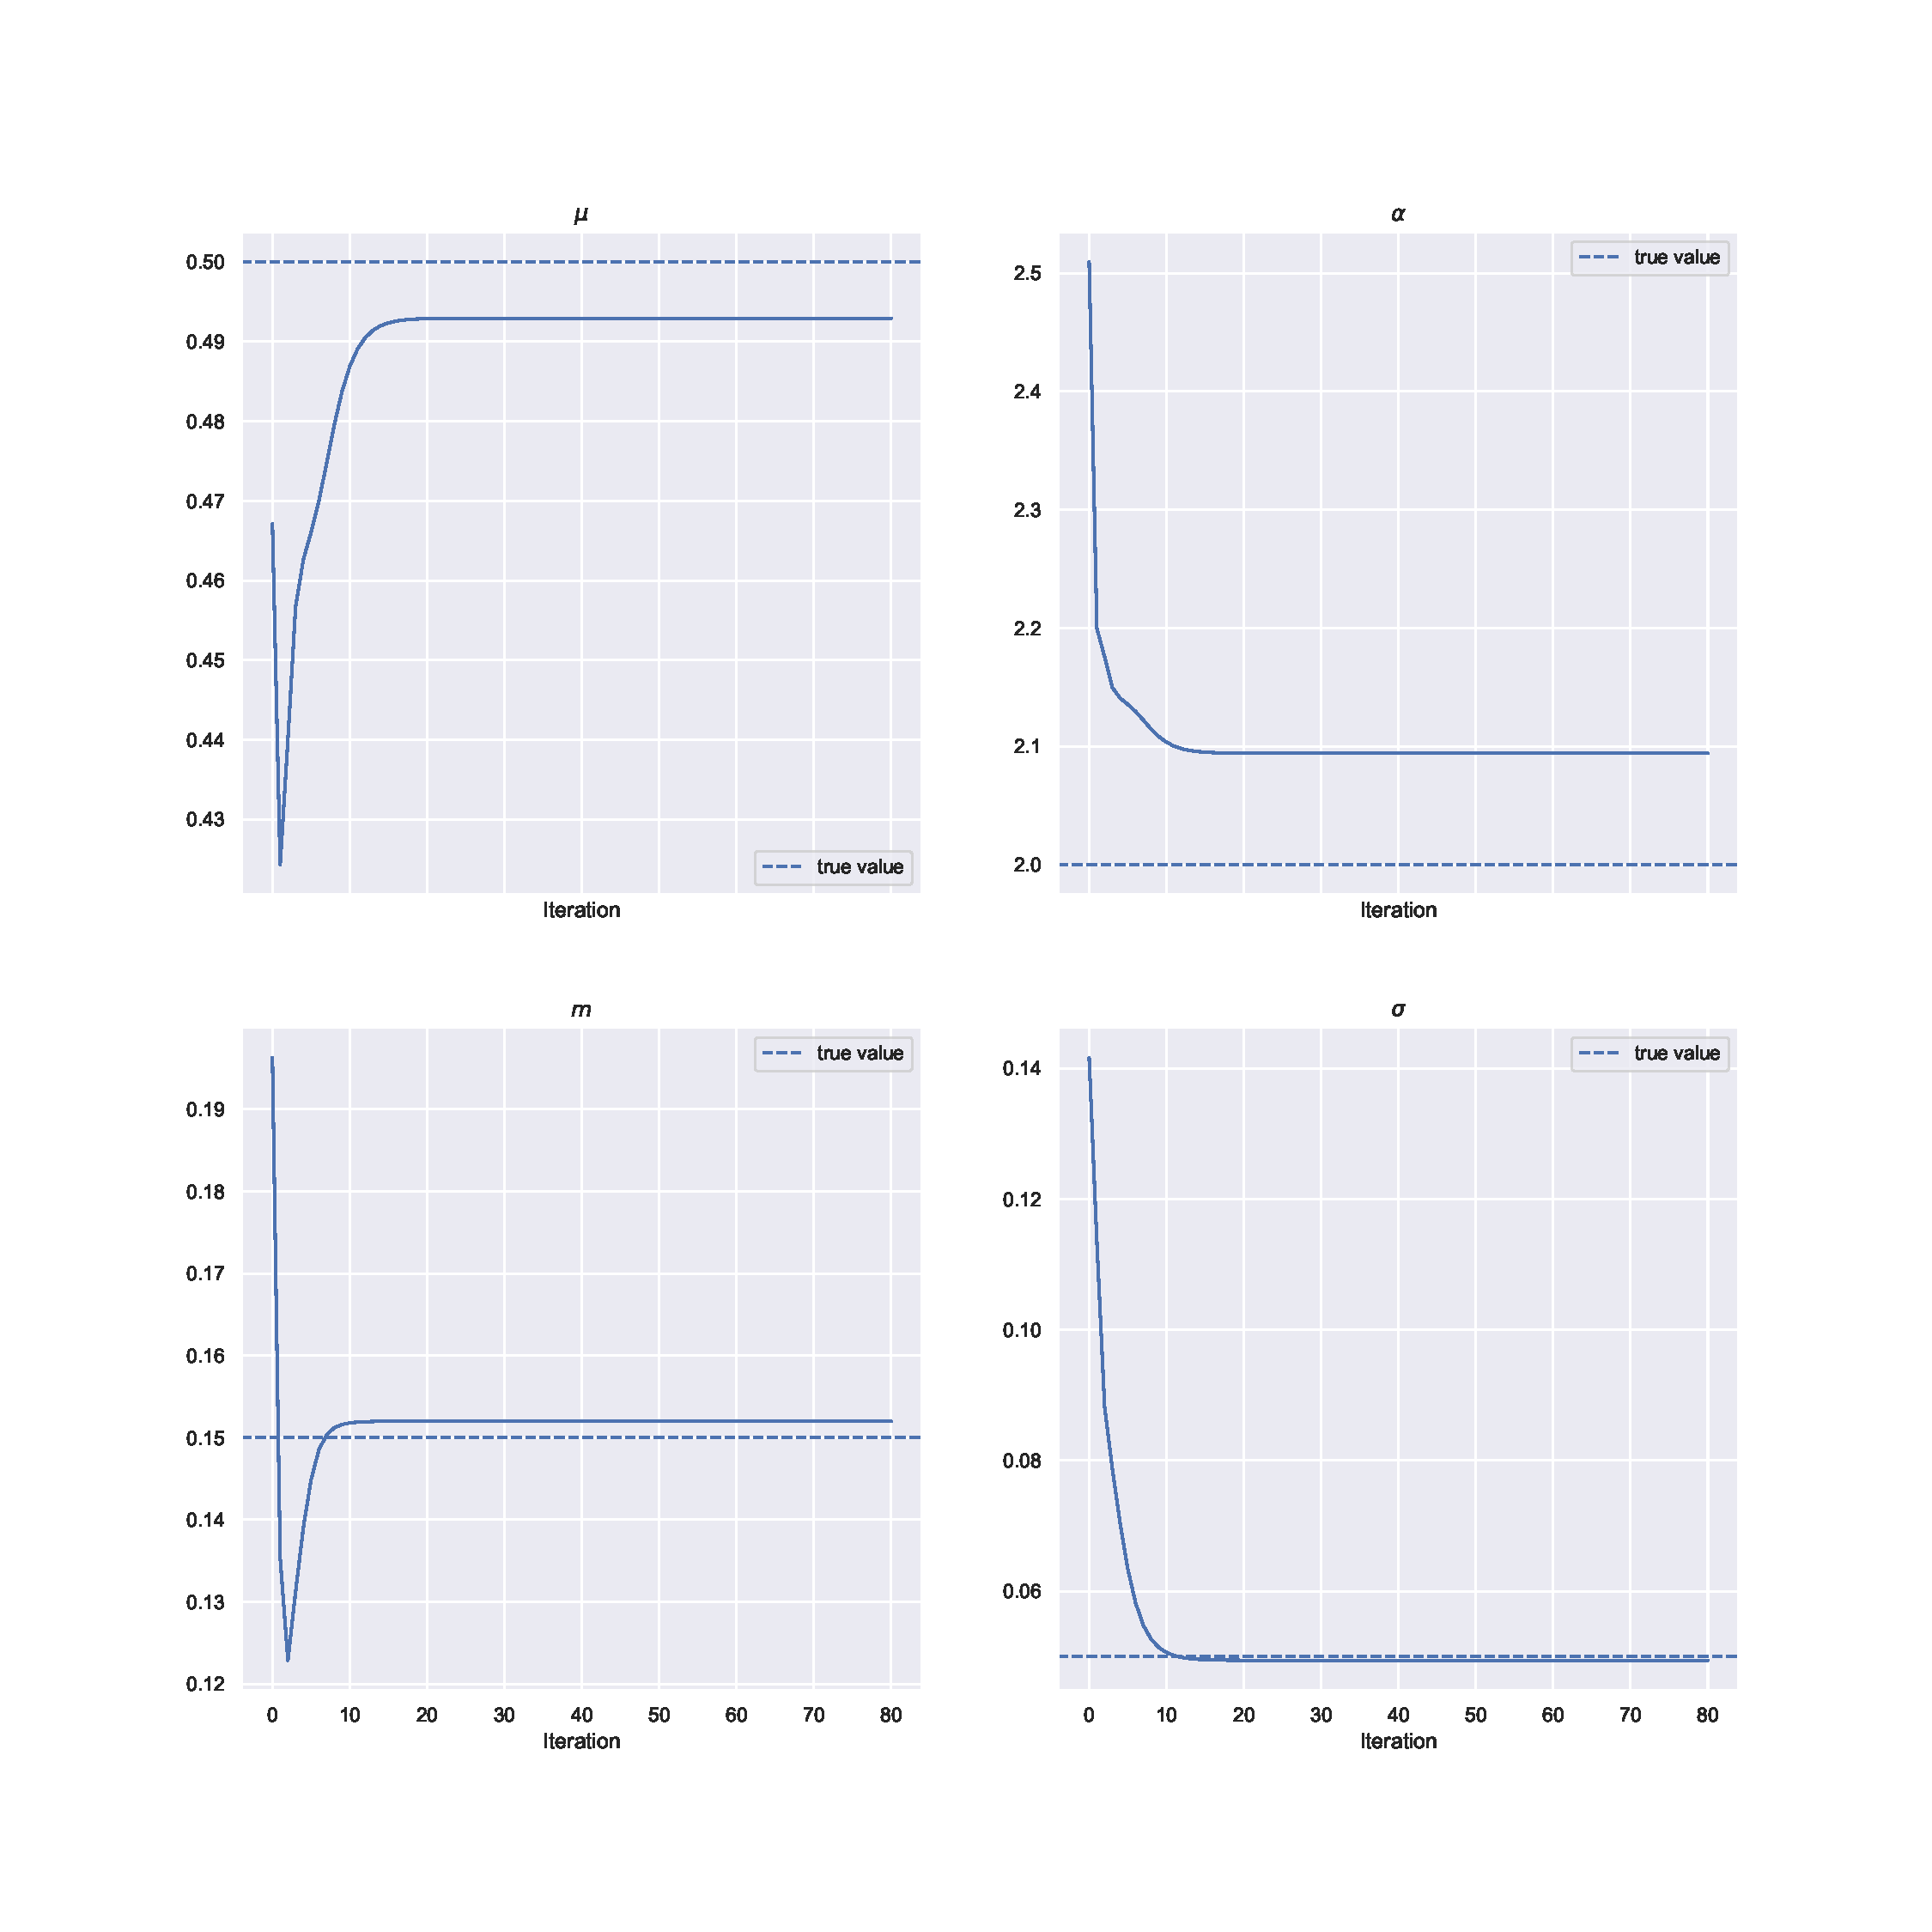
\includegraphics[width=\textwidth]{pics/results/history_params.pdf}
    \caption{Parameters recovery over 80 iterations with a \textit{smart} initialisation, on simulated data with $T = \SI{4}{\minute}$, $\texttt{isi}=\SI{1.2}{\second}$, $\texttt{n\_tasks} = \SI{80}{\percent}$, $\intervalleFF{a}{b} = \intervalleFF{30}{800}\times \SI{e-3}{\second}$.}
    \label{fig:history_params_1}
\end{figure}

Another experimentation of interest is to determine what is the influence of the hyper-parameters on the algorithm's capacity to converge toward the true value of the parameters.
In order to continue to generate data similar to a real M/EEG recording, in the following, unless otherwise stated, the inter-stimulus interval and the truncation values will be kept to reasonable values, i.e., $\texttt{isi}=\SI{1.2}{\second}$ and $\intervalleFF{a}{b} = \intervalleFF{30}{800}\times \SI{e-3}{\second}$.
Thus, the two main hyper-parameters we are interested in are the duration of the experimentation $T$ and the number of tasks timestamps kept \texttt{n\_tasks}.
This will allow us to see whether or not the algorithm needs a lot data to be efficient, both in term of duration or simply in absolute value.
This is a crucial point to determine as in reality, M/EEG data are costly to acquire, generally are of a relatively short duration, and the stimuli exerted on the subject count only a few repetitions per type, a hundred in the best of cases.

For those experimentations, we make \texttt{n\_tasks} and $T$ vary, keeping fixed all other parameters.
For every value of \texttt{n\_tasks} and $T$, we run 50 EM algorithms with 80 iterations, and plot the boxplots of the estimated parameters $\mu$, $\alpha$, $m$ and $\sigma$, with their true value, alongside the boxplots for the squared error of the loss and for the computation time of one EM simulation.
Results are shown in Fig.~\ref{fig:influence_of_n_tasks} and~\ref{fig:influence_of_T}.

\begin{figure}[h!]
    \centerfloat
    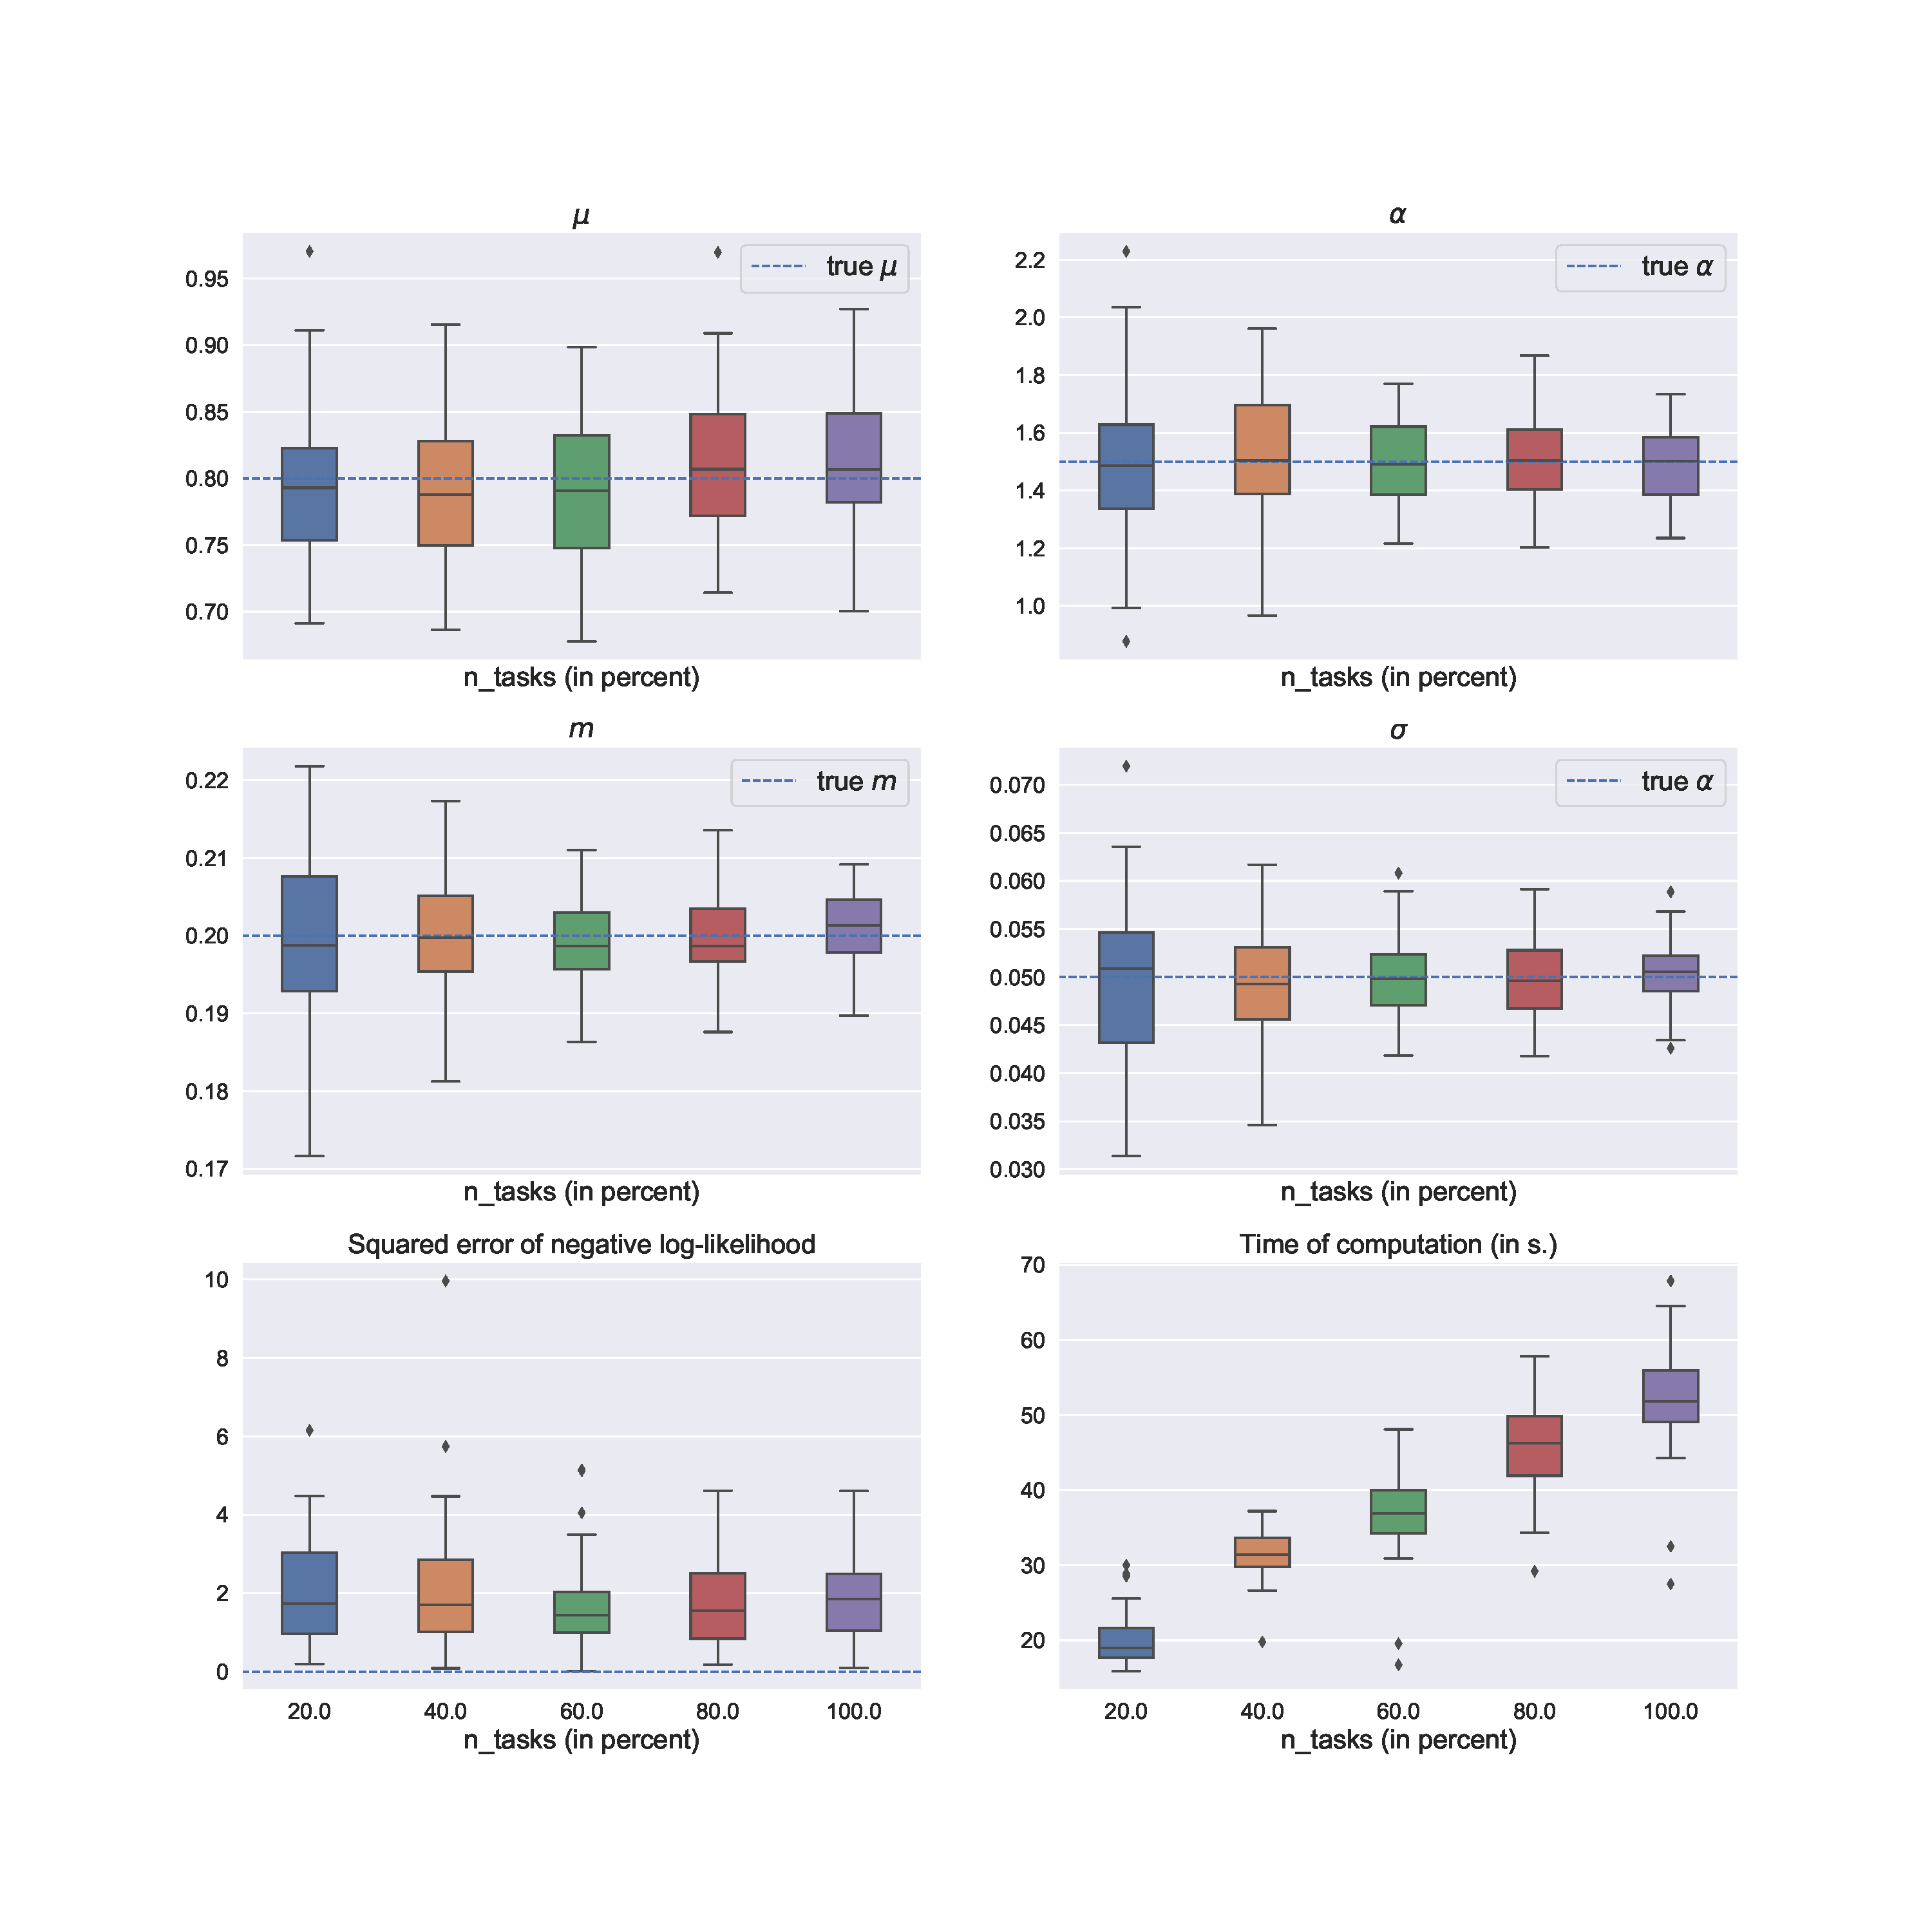
\includegraphics[width=1.28\textwidth]{pics/results/influence_of_n_tasks.pdf}
    \caption{Influence of \texttt{n\_tasks} on parameters recovery, loss error and computation time, 50 simulations for each value, with 80 EM iterations with a \textit{smart} initialisation, on simulated data with $T = \SI{4.6}{\minute}$, $\texttt{isi}=2.5$,, $\intervalleFF{a}{b} = \intervalleFF{30}{800}\times \SI{e-3}{\second}$.}
    \label{fig:influence_of_n_tasks}
\end{figure}

\begin{figure}[h!]
    \centerfloat
    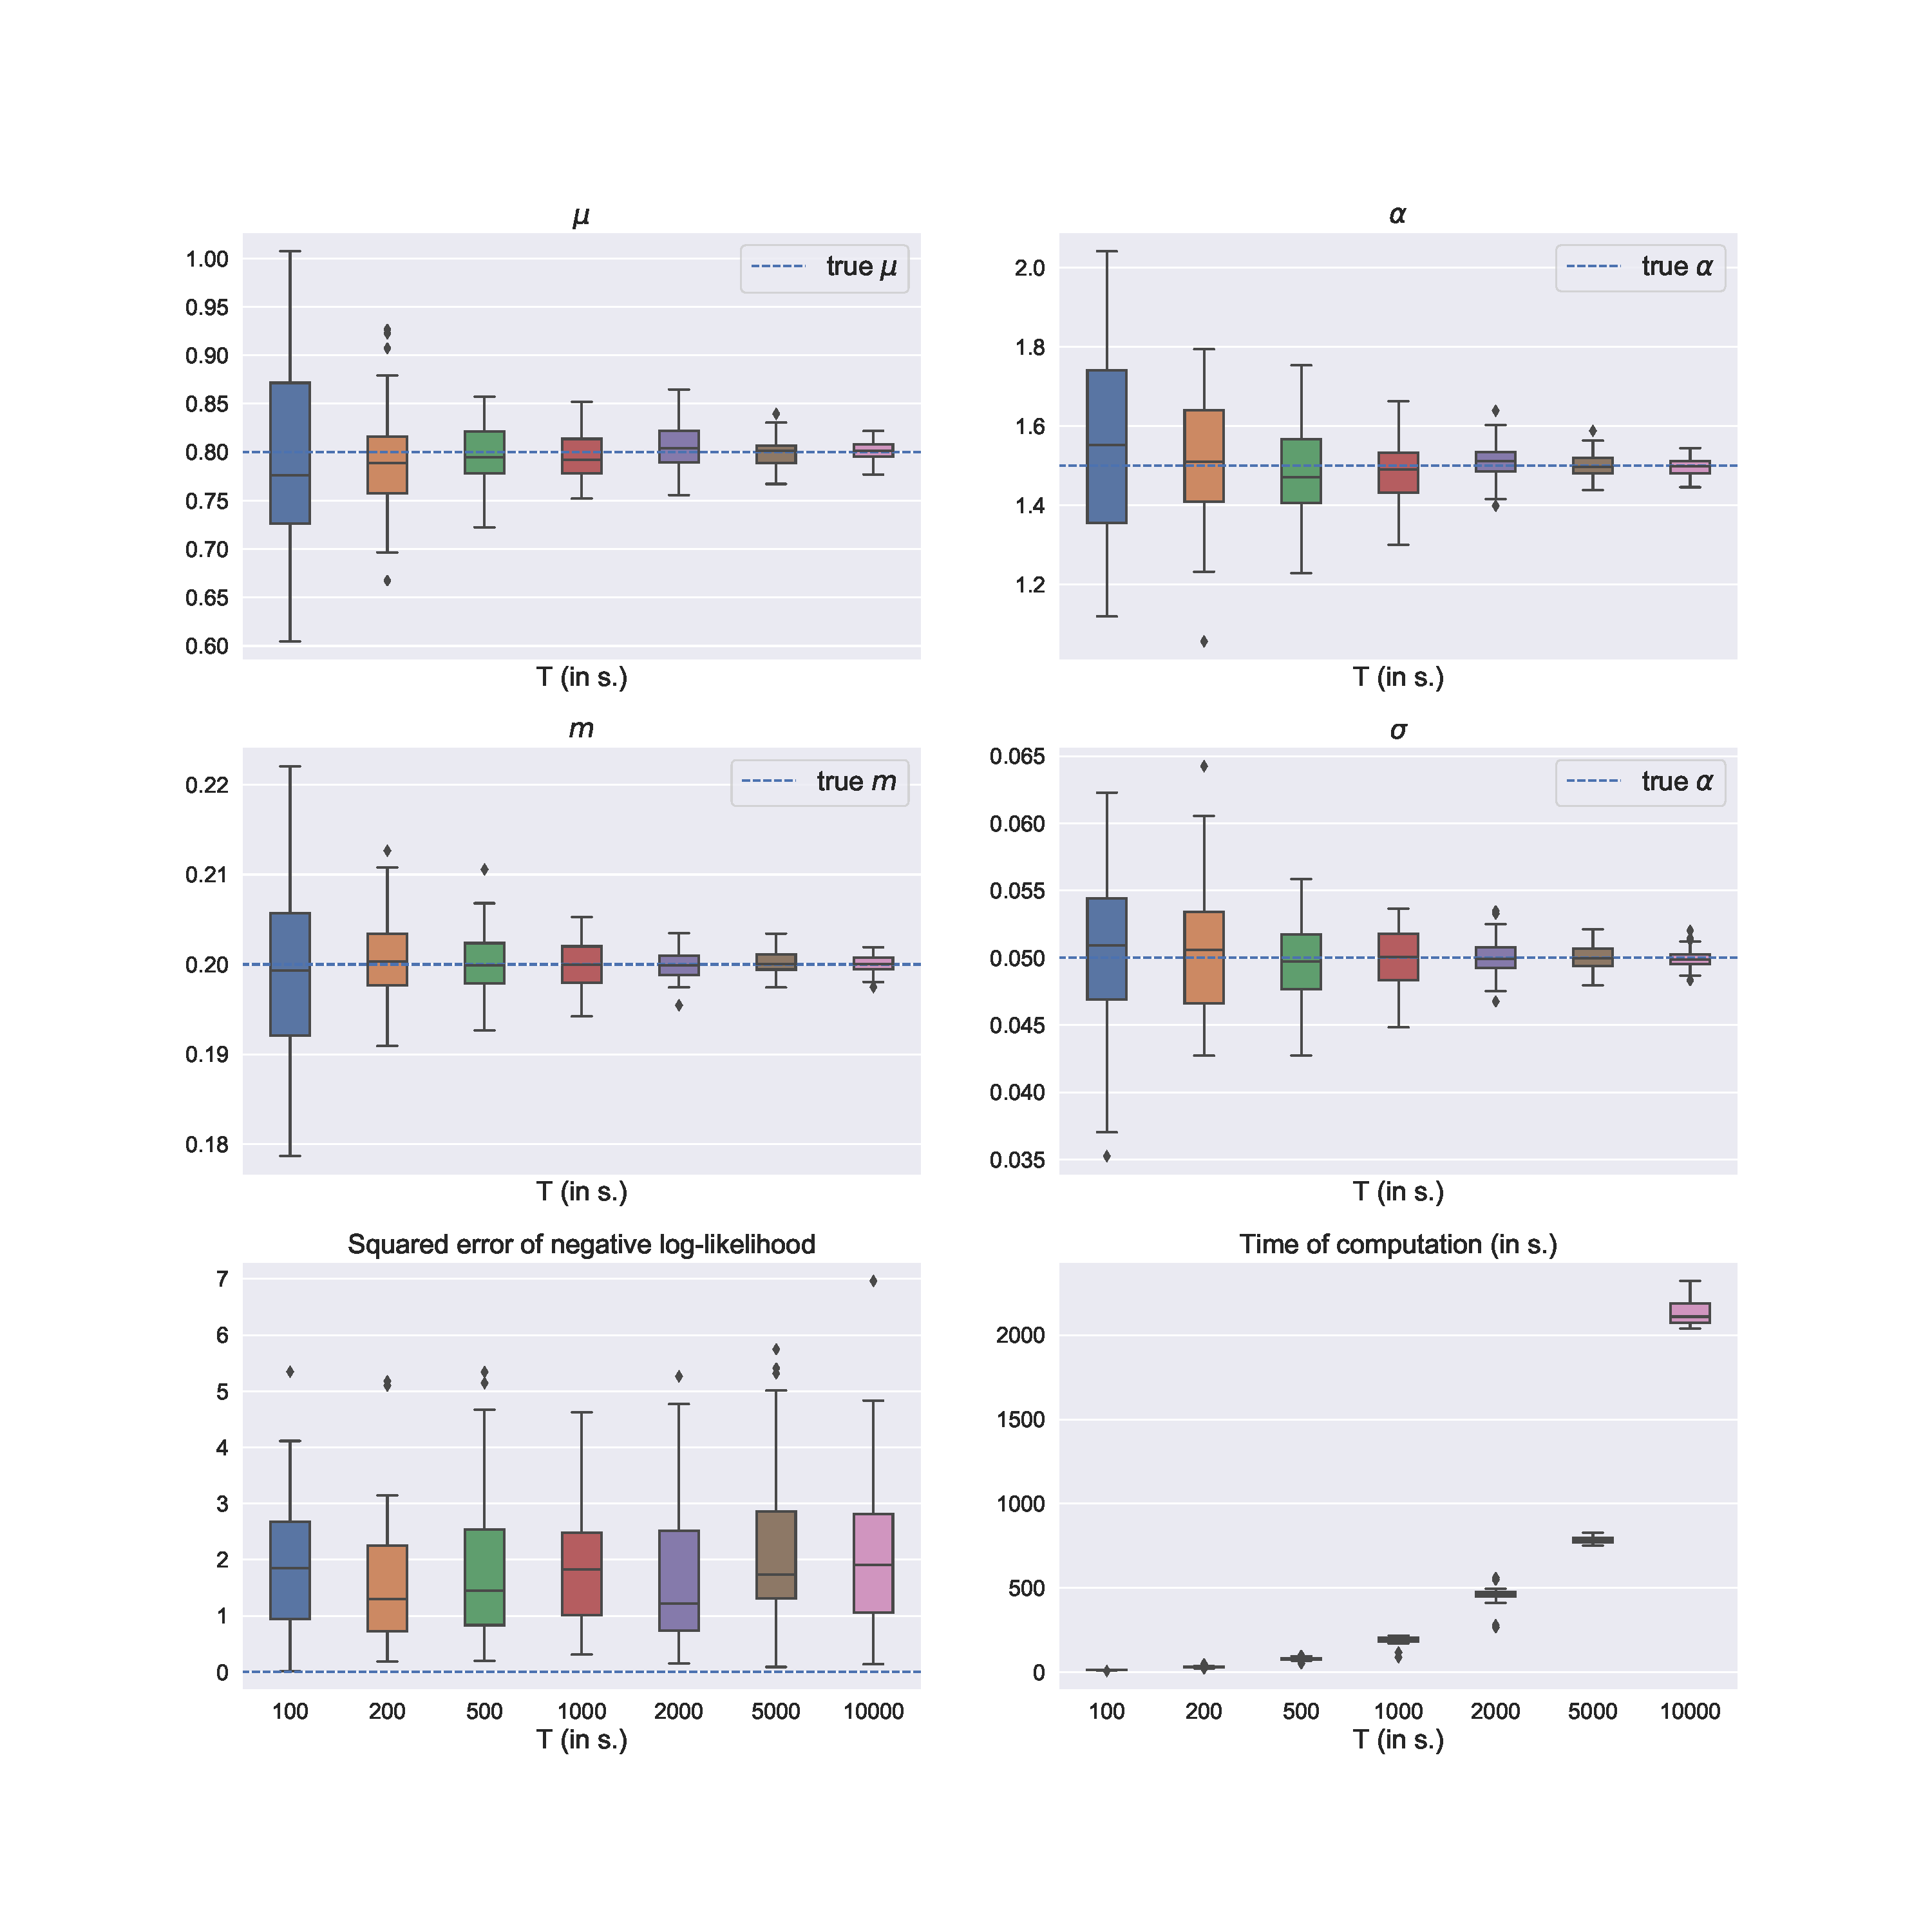
\includegraphics[width=1.28\textwidth]{pics/results/influence_of_T.pdf}
    \caption{Influence of $T$ on parameters recovery, loss error and computation time, 50 simulations for each value, with 80 EM iterations with a \textit{smart} initialisation, on simulated data with $\texttt{n\_tasks} = \SI{80}{\percent}$, $\texttt{isi}=2.5$,, $\intervalleFF{a}{b} = \intervalleFF{30}{800}\times \SI{e-3}{\second}$.}
    \label{fig:influence_of_T}
\end{figure}

